\documentclass[aspectratio=169]{beamer}
\usetheme{Madrid} % 主题
\usepackage[utf8]{inputenc}
\usepackage[T1]{fontenc}
\def\pgfsysdriver{pgfsys -dvipdfmx.def}
\usepackage{tikz}
\usepackage{graphicx}
\usepackage{url}
\usepackage{booktabs}
\usepackage{listings}
\definecolor{codegreen}{rgb}{0,0.6,0}
\definecolor{codegray}{rgb}{0.5,0.5,0.5}
\definecolor{codepurple}{rgb}{0.58,0,0.82}
\definecolor{backcolour}{rgb}{0.95,0.95,0.92}
\lstdefinestyle{mystyle}{
    backgroundcolor=\color{backcolour},   
    commentstyle=\color{codegreen},
    keywordstyle=\color{magenta},
    numberstyle=\tiny\color{codegray},
    stringstyle=\color{codepurple},
    basicstyle=\ttfamily\footnotesize,
    breakatwhitespace=false,         
    breaklines=true,                 
    captionpos=b,                    
    keepspaces=true,                 
    numbers=left,                    
    numbersep=5pt,                  
    showspaces=false,                
    showstringspaces=false,
    showtabs=false,                  
    tabsize=2
}
\lstset{style=mystyle}

% Title
\title[Containers \& VTs]{{Containers and Virtualization Technologies}}
%\subtitle{SubTitle}
\author[H. Suzumiya]{Hideo Suzumiya (Gaoyang Wei)}
\institute[Yangzhou University]{College of Information Engineering (College of Artificial Intelligence)}
\date[\today]{\today}

\begin{document}

\begin{frame}
\titlepage
\end{frame}

\begin{frame}
\frametitle{Outline}
\tableofcontents
\end{frame}

\section{Introduction}

\begin{frame}
\frametitle{Introduction}

{\Large \textbf{What is Virtualization ?}} \\
\textrm{Virtualization is a technology that allows \textsf{multiple virtual instances} of hardware, operating systems, and software applications to run on \textsf{a single physical server}, creating a virtual environment that appears to be a separate and independent computer system.} \\ \ \\
{\Large \textbf{5 Levels of Virtualization Technologies}}
\textrm{\begin{itemize}
\item Instruction Set Architecture Level \  \textit{e.g.} \textsf{QEMU}
\item Hardware Abstraction Level \  \textit{e.g.} \textsf{VMWare ESXi, Microsoft Hyper-V, KVM}
\item Operating System Level \  \textit{e.g.} \textsf{LXC, Docker}
\item Programming Language Level \  \textit{e.g.} \textsf{JVM, Microsoft dotNet}
\item Library Level \  \textit{e.g.} \textsf{Wine, WSL1}
\end{itemize}}

\end{frame}

\section{Background}

\begin{frame}[t]
\frametitle{Background}
{\Large Evolution of Virtualization} \\
{\ }\\
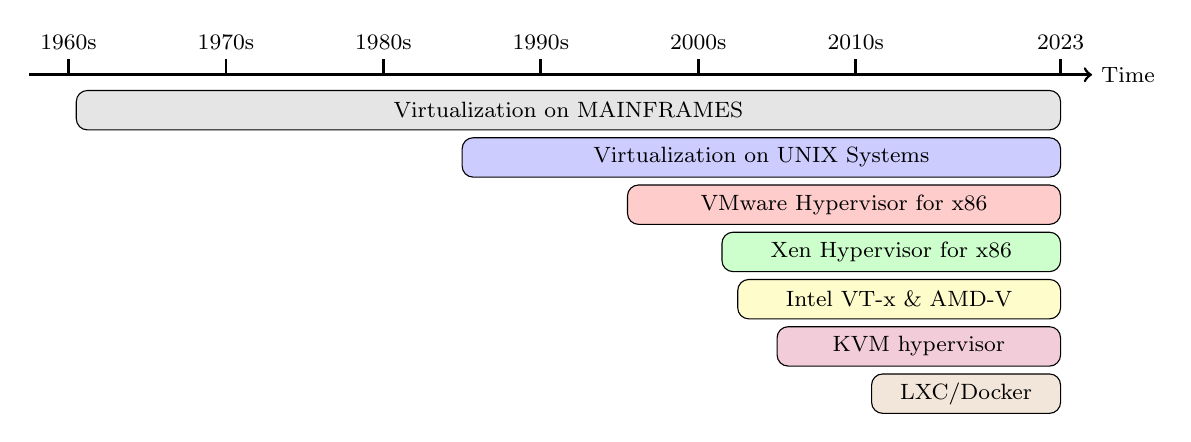
\begin{tikzpicture}
  % Draw timeline
  \footnotesize
  \draw[line width=1pt, ->] (0,0)--(13.5,0) node[right] {Time};
  \draw[line width=1pt] (0.5,0)-- (0.5,0.2) node[above] {1960s};
  \draw[line width=1pt] (2.5,0)-- (2.5,0.2) node[above] {1970s};
  \draw[line width=1pt] (4.5,0)--(4.5,0.2) node[above] {1980s};
  \draw[line width=1pt] (6.5,0)--(6.5,0.2) node[above] {1990s};
  \draw[line width=1pt] (8.5,0)--(8.5,0.2) node[above] {2000s};
  \draw[line width=1pt] (10.5,0)--(10.5,0.2) node[above] {2010s};
  \draw[line width=1pt] (13.1,0)--(13.1,0.2) node[above] {2023};
  % Draw rectangles
  \draw[rounded corners, fill=gray!20] (0.6,-0.2) rectangle (13.1,-0.7) node[midway] {Virtualization on MAINFRAMES};
  \draw[rounded corners, fill=blue!20] (5.5,-0.8) rectangle (13.1,-1.3) node[midway] {Virtualization on UNIX Systems};
  \draw[rounded corners, fill=red!20] (7.6,-1.4) rectangle (13.1,-1.9) node[midway] {VMware Hypervisor for x86};
  \draw[rounded corners, fill=green!20] (8.8,-2) rectangle (13.1,-2.5) node[midway] {Xen Hypervisor for x86};
  \draw[rounded corners, fill=yellow!20] (9.0,-2.6) rectangle (13.1,-3.1) node[midway] {Intel VT-x \& AMD-V};
  \draw[rounded corners, fill=purple!20] (9.5,-3.2) rectangle (13.1,-3.7) node[midway] {KVM hypervisor};
  \draw[rounded corners, fill=brown!20] (10.7,-3.8) rectangle (13.1,-4.3) node[midway] {LXC/Docker};
\end{tikzpicture}
\end{frame}


\begin{frame}[t]
\frametitle{Background}
{\Large Cloud Computing Models} \\ \ \\
\begin{figure}
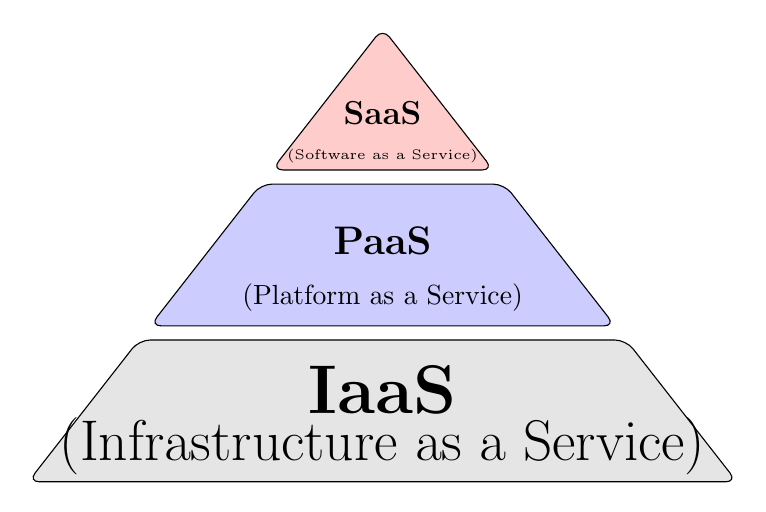
\begin{tikzpicture}[scale=0.9]
\draw[rounded corners, fill=red!20] (3.4375,-2) -- (5,0)-- (6.5625,-2) -- cycle;
\node at (5,-1.2) [anchor=center] {\large \textbf{SaaS}};
\node at (5,-1.8) [anchor=center] {\tiny (Software as a Service)};

\draw[rounded corners, fill=blue!20] (1.71875,-4.2) -- (3.28125,-2.2) -- (6.71875,-2.2) -- (8.28125,-4.2) -- cycle;
\node at (5,-3) [anchor=center] {\Large \textbf{PaaS}};
\node at (5,-3.8) [anchor=center] {(Platform as a Service)};

\draw[rounded corners, fill=gray!20] (0,-6.4) -- (1.5625,-4.4) -- (8.4375,-4.4) -- (10,-6.4) -- cycle;
\node at (5,-5.1) [anchor=center] {\Huge \textbf{IaaS}};
\node at (5,-5.9) [anchor=center] {\huge (Infrastructure as a Service)};
\end{tikzpicture}
\end{figure}
\end{frame}

\section{Virtualization}

\begin{frame}
\frametitle{Virtualization}
\textrm{\begin{itemize}
\item Virtualization enables multiple virtual machines (VMs) to run on a single physical server, each with its own operating system and applications.
\item Virtualization provides a way to consolidate servers, reduce hardware costs, and increase resource utilization.
\item Popular virtualization platforms include \textsf{VMware, Hyper-V, and Kernel-based Virtual Machine}.
\end{itemize}}
\end{frame}

\begin{frame}[t]
\frametitle{Virtualization}
{\Large KVM \& Hyper-V Architectures \\}
\begin{figure}[htbp]
\centering
\includegraphics[scale=0.28]{img/Kernel-based_Virtual_Machine.pdf}
\qquad
\includegraphics[scale=0.323]{img/Hyper-V.png}
\end{figure}
\end{frame}

\begin{frame}[t]
\frametitle{Virtualization}
\begin{figure}[htbp]
\centering
\includegraphics[scale=0.16]{img/proxmox-ve.png}
\caption{Proxmox VE 7.3 based on KVM and LXC}
\end{figure}
\end{frame}

\section{Containers}

\begin{frame}
\frametitle{Containers}
{\Large \textbf{What is Container?}}
\textrm{\begin{itemize}
	\item Containers provide a way to package and deploy applications in a lightweight, portable, and reproducible way.
	\item \textsf{Containers} are Operating System Level VMs!
	\item \textsf{Docker} is a popular containerization platform that enables developers to build, ship, and run distributed applications in containers.
\end{itemize}}
{\Large \textbf{Philosophy of Docker}}
\textrm{\begin{itemize}
	\item Write once, run everywhere.
	\item One container runs one application.
\end{itemize}}
\end{frame}

\begin{frame}
\frametitle{Containers}
\begin{figure}[htbp]
\centering
\includegraphics[scale=0.47]{img/docker-architecture.pdf}
\caption{Docker Architecture}
\end{figure}
\end{frame}

\section{Comparison}

\begin{frame}
\frametitle{Comparison}
{\Large \textbf{Containers V.S. VMs}}
	\begin{figure}
		\center
		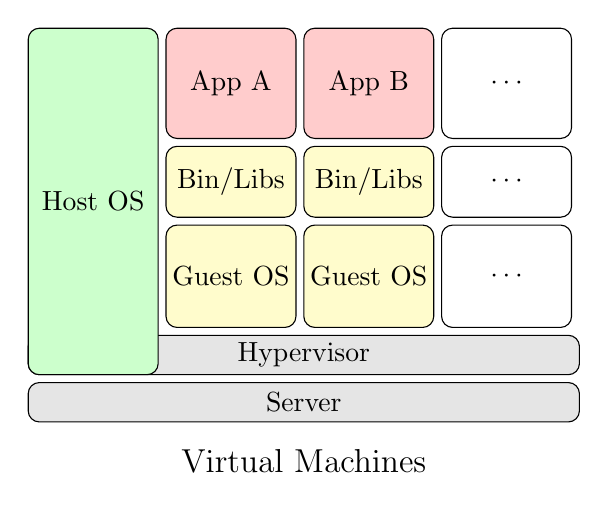
\begin{tikzpicture}
			\node at (3.5,-0.5) [anchor=center] {\large Virtual Machines};
			\draw[rounded corners, fill=gray!20]   (0,    0.0) rectangle (7,    0.5) node[midway] {Server};
			\draw[rounded corners, fill=gray!20]   (0,    0.6) rectangle (7,    1.1) node[midway] {Hypervisor};
			\draw[rounded corners, fill=green!20]  (0,    0.6) rectangle (1.65, 5)   node[midway] {Host OS};
			\draw[rounded corners, fill=yellow!20] (1.75, 1.2) rectangle (3.4,  2.5) node[midway] {Guest OS};
			\draw[rounded corners, fill=yellow!20] (3.5,  1.2) rectangle (5.15, 2.5) node[midway] {Guest OS};
			\draw[rounded corners]                 (5.25, 1.2) rectangle (6.9,  2.5) node[midway] {$\cdots$};
			\draw[rounded corners, fill=yellow!20] (1.75, 2.6) rectangle (3.4,  3.5) node[midway] {Bin/Libs};
			\draw[rounded corners, fill=yellow!20] (3.5,  2.6) rectangle (5.15, 3.5) node[midway] {Bin/Libs};
			\draw[rounded corners]                 (5.25, 2.6) rectangle (6.9,  3.5) node[midway] {$\cdots$};
			\draw[rounded corners, fill=red!20]    (1.75, 3.6) rectangle (3.4,  5)   node[midway] {App A};
			\draw[rounded corners, fill=red!20]    (3.5,  3.6) rectangle (5.15, 5)   node[midway] {App B};
			\draw[rounded corners]                 (5.25, 3.6) rectangle (6.9,  5)   node[midway] {$\cdots$};
		\end{tikzpicture}
		\quad
		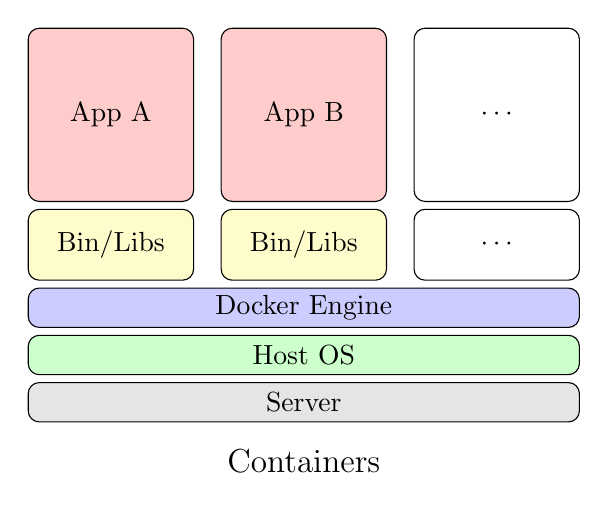
\begin{tikzpicture}
			\node at (3.5,-0.5) [anchor=center] {\large Containers};
			\draw[rounded corners, fill=gray!20]   (0,    0)   rectangle (7,    0.5) node[midway] {Server};
			\draw[rounded corners, fill=green!20]  (0,    0.6) rectangle (7,    1.1) node[midway] {Host OS};
			\draw[rounded corners, fill=blue!20]   (0,    1.2) rectangle (7,    1.7) node[midway] {Docker Engine};
			\draw[rounded corners, fill=yellow!20] (0,    1.8) rectangle (2.1,  2.7) node[midway] {Bin/Libs};
			\draw[rounded corners, fill=yellow!20] (2.45, 1.8) rectangle (4.55, 2.7) node[midway] {Bin/Libs};
			\draw[rounded corners]                 (4.9,  1.8) rectangle (7,    2.7) node[midway] {$\cdots$};
			\draw[rounded corners, fill=red!20]    (0,    2.8) rectangle (2.1,  5)   node[midway] {App A};
			\draw[rounded corners, fill=red!20]    (2.45, 2.8) rectangle (4.55, 5)   node[midway] {App B};
			\draw[rounded corners]                 (4.9,  2.8) rectangle (7,    5)   node[midway] {$\cdots$};
		\end{tikzpicture}
	\end{figure}
\end{frame}

\begin{frame}
\frametitle{Comparison}
	\begin{itemize}
		\item Containers are faster, more lightweight, and more efficient than VMs.
		\item VMs provide greater isolation and security than containers.
		\item Containers are better suited for microservices-based architectures, while VMs are better suited for legacy applications and monolithic architectures.
	\end{itemize}
	\begin{table}[hbp]
		\center
		\textrm{\begin{tabular}{ccc} \toprule
			Attribute          & Container           & VM \\ \midrule
			Start              & Seconds             & Minutes \\
			Size               & 10s of Megabytes    & 10s of Gigabytes \\
			Performance        & Close to native     & Weaker \\
			Supported Quantity & 1000s of containers & 10s of Guests \\ \bottomrule
		\end{tabular}}
		\caption{The comparison}
	\end{table}
\end{frame}

\section{Docker Practice}

\begin{frame}[fragile,t]
\frametitle{Install Docker}
{\Large \textbf{Steps of installing Docker on linux}}\\
Running Docker on Windows \& macOS is \textbf{NOT} recommended!
	\begin{itemize}
		\item Change source repo \\
		\verb+export DOWNLOAD_URL="https://mirrors.bfsu.edu.cn/docker-ce"+
		\item Use auto installation script \\
		\verb+curl -fsSL https://get.docker.com/ | sh+
		\item Or \\
		\verb+wget -O- https://get.docker.com/ | sh+
		\item Change DockerHub repo \\
		\verb+touch /etc/docker/daemon.json+
		\begin{verbatim}
			{
			  "registry-mirrors": [
			    "https://hub-mirror.c.163.com",
			    "https://mirror.baidubce.com" ]
			}
		\end{verbatim}
	\end{itemize}
\end{frame}

\begin{frame}[fragile,t]
\frametitle{Install Docker}
	\begin{itemize}
		\item Reload systemd services \\
		\verb+sudo systemctl daemon-reload+ \\
		\verb+sudo systemctl restart docker+
		\item Execute \verb+docker info+ and if you see \\
		\begin{verbatim}
			Registry Mirrors:
			 https://hub-mirror.c.163.com/
		\end{verbatim}
		The configuration has been applied.
	\end{itemize}
\end{frame}

\begin{frame}
\frametitle{Container Management}
\begin{table}[hbp]
		\center
		\begin{tabular}{ll}
			\toprule
			\textbf{Command} & \textbf{Description} \\
			\midrule
			\texttt{docker\ create} \textit{image} [\ \textit{command}\ ] &  Crete the container \\
			\texttt{docker\ run} \textit{image} [\ \textit{command}\ ]  & = \texttt{create} + \texttt{start}  \\ 
			\midrule
			\texttt{docker\ start} \textit{container} $\cdots$ & Start the container\\
			\texttt{docker\ stop} \textit{container} $\cdots$ & Graceful stop\\
			\texttt{docker\ kill} \textit{container} $\cdots$ & Kill (SIGKILL) the container\\
			\texttt{docker\ restart} \textit{container} $\cdots$ & = \texttt{stop} + \texttt{start} \\
			\midrule
			\texttt{docker\ pause} \textit{container} $\cdots$ & Suspend the container \\
			\texttt{docker\ unpause} \textit{container} $\cdots$ & Resume the container \\
			\midrule
			\texttt{docker\ rm} [\ \texttt{-f}\ ] \textit{container} $\cdots$ & Destroy the container \\
			\bottomrule
		\end{tabular}
	\end{table}
\end{frame}

\begin{frame}
\frametitle{Container Inspection}
	\begin{table}[hbp]
		\center
		\begin{tabular}{lp{21em}}
			\toprule
			\textbf{Command} & \textbf{Description} \\
			\midrule
			\texttt{docker\ ps} & List running containers\\
			\texttt{docker\ ps\ -a} & Lista all containers \\
			\texttt{docker\ logs} [\ \texttt{-f}\ ] \textit{container} $\cdots$ & Show the container output (stdout \& stderr) \\
			\texttt{docker\ top} \textit{container} [\ \textit{ps\ options}\ ] & List the process running inside the container \\
			\texttt{docker diff} \textit{container} & Show the difference with images (modified files) \\
			\texttt{docker inspect} \textit{container} $\cdots$ & Show low-level infos (in \texttt{json} format) \\
			\bottomrule
		\end{tabular}
	\end{table}
\end{frame}

\begin{frame}
\frametitle{Container intertraction}
	\begin{table}[hbp]
		\center
		\begin{tabular}{lp{21em}}
			\toprule
			\textbf{Command} & \textbf{Description} \\
			\midrule
			\texttt{docker\ attach} \textit{container} & attach to a running container (stdin/stdout/stderr) \\
			\texttt{docker\ cp} \textit{container:path hostpath}|- & Copy files from container \\
			\texttt{docker\ cp} \textit{hostpath}|- \textit{container:path} & Copy files to container \\
			\texttt{docker\ export} \textit{container} & export the content of the container (Tar archive) \\
			\texttt{docker exec} \textit{container} $\cdots$ & Run a command in an existing container \\
			\texttt{docker wait} \textit{container} & Wait until the container terminates and return the exit code \\
			\texttt{docker commit} \textit{container image} & Commit a new docker image (snapshot or container) \\
			\bottomrule
		\end{tabular}
	\end{table}
\end{frame}

\begin{frame}
\frametitle{Image management}
	\begin{table}[hbp]
		\center
		\begin{tabular}{lp{21em}}
			\toprule
			\textbf{Command} & \textbf{Description} \\
			\midrule
			\texttt{docker\ images} & List all local images \\
			\texttt{docker\ history} \textit{image} & Show image history (list of ancestors) \\
			\texttt{docker\ inspect} \textit{image} $\cdots$ & Show low-level infos (in \texttt{json} format) \\
			\midrule
			\texttt{docker\ tag} \textit{image tag} & Tag an image \\
			\midrule
			\texttt{docker\ commit} \textit{container image} & Create image from container \\
			\texttt{docker\ import} \textit{url}|- [\textit{tag}] & Create image from tarball \\
			\midrule
			\texttt{docker\ rmi} \textit{image} $\cdots$ & Delete images \\
			\bottomrule
		\end{tabular}
	\end{table}
\end{frame}

\begin{frame}
\frametitle{Image transfer}
	\begin{table}[hbp]
		\center
		\begin{tabular}{lp{21em}}
			\toprule
			\textbf{Command} & \textbf{Description} \\
			\midrule
			\texttt{docker pull} \textit{repo}[:\textit{tag}] $\cdots$
				& Pull an image/repo from a registry \\
			\texttt{docker push} \textit{repo}[:\textit{tag}] $\cdots$
				& Push an image/repo from a registry \\
			\texttt{docker search} \textit{text}
				& Search an image from the official registry \\
			\midrule
			\texttt{docker login} $\cdots$ & Login to a registry \\
			\texttt{docker logout} $\cdots$ & Logout from a registry \\
			\bottomrule
		\end{tabular}
		\caption{Using the registry API}
	\end{table}
\end{frame}

\begin{frame}
\frametitle{Image transfer}
	\begin{table}[hbp]
		\center
		\begin{tabular}{lp{21em}}
			\toprule
			\textbf{Command} & \textbf{Description} \\
			\midrule
			\texttt{docker save} \textit{repo}[:\textit{tag}] $\cdots$
				& Export an image/repo as a tarball \\
			\texttt{docker load} & Load image from a tarball \\
			\midrule
			\texttt{docker-ssh} $\cdots$ & Proposed script to transfer images between 2 daemons over ssh \\
			\bottomrule
		\end{tabular}
		\caption{Manual transfer}
	\end{table}
\end{frame}

\begin{frame}
\frametitle{Builder}
	\begin{table}[hbp]
		\center
		\begin{tabular}{lp{21em}}
			\toprule
			\textbf{Command} & \textbf{Description} \\
			\midrule
			\texttt{FROM} \textit{image}|\textit{scratch}
				& Base image for the build \\
			\texttt{MAINTAINER} \textit{email}
				& Name of maintainer (metadata) \\
			\midrule
			\texttt{COPY} \textit{path dst}
				& Copy \textit{path} from the context into the container at location \textit{dst} \\
			\texttt{ADD} \textit{src dst}
				& Same as \texttt{COPY} but untar archives and accepts http urls \\
			\texttt{RUN} \textit{args} $\cdots$
				& Run an arbitrary command inside the container \\
			\midrule
			\texttt{USER} \textit{name}
				& Set the default username \\
			\texttt{WORKDIR} \textit{path}
				& Set the default working directory \\
			\texttt{CMD} \textit{args} $\cdots$
				& Set the default command \\
			\texttt{ENV} \textit{name value}
				& Set environment variables \\
			\bottomrule
		\end{tabular}
	\end{table}
\end{frame}

\section{Conclusion}

\begin{frame}
	\frametitle{Conclusion}
	\begin{itemize}
		\item Containerization and virtualization are both important technologies for modern application development and deployment.
		\item Containers and VMs have different strengths and weaknesses, and choosing the right technology depends on the specific requirements of the application and infrastructure.
	\end{itemize}
\end{frame}

\begin{frame}
	\frametitle{Conclusion}
	\begin{figure}[htbp]
		\centering
		\includegraphics[scale=0.2]{img/docker-cheatsheet.png}
		\caption{Docker Cheatsheet: https://raw.githubusercontent.com/sangam14/dockercheatsheets/master/dockercheatsheet8.png}
	\end{figure}
\end{frame}

\begin{frame}
	\begin{center}
	\fontsize{72pt}{\baselineskip}\selectfont\textbf{Thanks!}
	\end{center}
\end{frame}

\end{document}